%%%%%%%%%%%%%%%%%%%%%%%%%%%%%%%%%%%%%%%%%%%%%%%%%%%%%%%%%%%%%%%%%%%%%%%%%%%%%%%%
%2345678901234567890123456789012345678901234567890123456789012345678901234567890
%        1         2         3         4         5         6         7         8

\documentclass[letterpaper, 10 pt, conference]{ieeeconf}  % Comment this line out
                                                          % if you need a4paper
%\documentclass[a4paper, 10pt, conference]{ieeeconf}      % Use this line for a4
                                                          % paper

\IEEEoverridecommandlockouts                              % This command is only
                                                          % needed if you want to
                                                          % use the \thanks command
\overrideIEEEmargins
% See the \addtolength command later in the file to balance the column lengths
% on the last page of the document

\usepackage[utf8]{inputenc}
\usepackage[T1]{fontenc}
\usepackage{float}
\usepackage{pgfplots}
\pgfplotsset{width=8cm,compat=1.9}

% The following packages can be found on http:\\www.ctan.org
%\usepackage{graphics} % for pdf, bitmapped graphics files
%\usepackage{epsfig} % for postscript graphics files
%\usepackage{mathptmx} % assumes new font selection scheme installed
%\usepackage{mathptmx} % assumes new font selection scheme installed
%\usepackage{amsmath} % assumes amsmath package installed
%\usepackage{amssymb}  % assumes amsmath package installed

\title{\LARGE \bf
SoK: Classifying Honeypot Fingerprinting Techniques
}

%%%% For Double Blind Version
%\author{Shreyas Srinivasa$^{1}$, Emmanouil Vasilomanolakis$^{2}$, Jens Myrup Pedersen$^{3}$% <-this % stops a space
%\thanks{*This work was not supported by any organization}% <-this % stops a space
%\thanks{$^{1}$S. Srinivasa - PhD Fellow at Department of Electronic Systems,
%        Aalborg University, Copenhagen, Denmark
%        {\tt\small shsr@es.aau.dk}}%
%\thanks{$^{2,3}$E. Vasilomanolakis, J. Pedersen - Asst. Professor at                          Department of Electronic Systems, Aalborg University,                         Copenhagen, Denmark
%        {\tt\small emv@es.aau.dk, jens@es.aau.dk}}%
%}


\begin{document}



\maketitle
\thispagestyle{empty}
\pagestyle{empty}


%%%%%%%%%%%%%%%%%%%%%%%%%%%%%%%%%%%%%%%%%%%%%%%%%%%%%%%%%%%%%%%%%%%%%%%%%%%%%%%%
\begin{abstract}
In defensive security, Honeypots play an important role to detect attacks by simulating the services of the target system. Over the years, many honeypots have been proposed, developed and deployed over the internet simulating essential protocols and services like HTTP, SSH, Telnet, SMB, SMTP, FTP and also industrial protocols like MODBUS and BARCnet. Survey statistics provided by F-Secure (rfr: F-secure white paper), show that the attack landscape caught by honeypots hosted by F-Secure, have tripled from 2018 with major targeted protocols being Telnet, SMB, SSH and  MSSQL. The rise in attacks can be in view of increase in smart IoT devices and also the accessibility of Cloud infrastructure. Further, resource constraints on IoT devices lead to poor security diligence to achieve performance and availability. Honeypots have been a reliable choice for proactive defense by  network administrators to detect and analyze attacks. Open-source low-interaction honeypots like Kippo, Cowrie, Glastopf, Dionaea and Conpot are the most widely deployed Honeypots (rfr: bitter harvest). As effective as  honeypots can be leveraged to detect attacks, they are also vulnerable to be exposed as decoys thereby reducing their productivity. The identity of honeypots and its ability to remain undetected is a valuable parameter towards its purpose. Studies have shown that these honeypots are easily detectable and can be fingerprint by various mechanisms. Probing, response analysis and  location/domain filtering are some methods through which the identity of honeypots can be revealed. In addition, machine learning based methods have inferred to increase the predictability and reduce false positives in detection. This paper provides an overview and a new basis for classification of honeypot fingerprinting mechanisms . 
\end{abstract}


%%%%%%%%%%%%%%%%%%%%%%%%%%%%%%%%%%%%%%%%%%%%%%%%%%%%%%%%%%%%%%%%%%%%%%%%%%%%%%%%
\section{INTRODUCTION}

The rise of Internet of Things and affordable cloud infrastructure has led to a connected world of devices and services working together to achieve better accessibility and connectivity in real time. While these devices are resource constrained, there is more focus on performance and availability rather on security. Also, accessibility being important, leads to various services open to the internet thereby creating a huge risk in security of the system. Leveraging these known vulnerabilities, proactive security strategies like Honeypots are developed and deployed with these flaws to attract exploits from attackers thereby making them vulnerable by design.Honeypots are classified into three types based on their interaction, service simulation into low, medium and high interaction honeypots. As the name suggests, low interaction honeypots are focused on emulating the basic protocol services and do not focus on high interaction. Low interaction honeypots are quick to setup, highly usable and provide basic logging and analysis features. These honeypots are developed  to be deployed in resource constraint environments and basically perform event logging. Low interaction honeypots are also not security critical as any damage caused by them as a result of exploitation are minimal 

In addition to various security measures adopted by the administrators, Honeypots form a good defensive tool as decoy systems, to identify vulnerabilities and detect attacks. They act as a proactive approach to identify malicious sources for attacks and also give an understanding of the vulnerable areas of the system. All communication to the honeypot is considered hostile, since legitimate users have no obligation to access a honeypot. The use of honeypots as a detection tool date back to over a decade with honeypot projects being open and deployed since the year 2000. Protocols like Telnet and SSH have been widely used even today to establish communication with remote systems. Similarly protocols like HTTP, FTP, SMTP, SNMP, SMB have been the used as base network communication protocols for essential services. There are honeypots developed to emulate all the stated essential protocols. The Honeynet Project \cite{Honeynet} is focused on development of honeypots for well known protocols and environments over the years. Administrators have been using these honeypot projects in their DMZ environments to detect the attacks on these protocols over years. However, it has been evident that these honeypots could be detected and identified. This leads to an argument about the use of outdated honeypots and their contribution towards attack detection once they are identified.

Honeypot detection is important to notify the developers of these projects of the maintenance. Soon after these projects are released as open source, very little attention is given to updating or patching. While, bad maintenance of any software is a huge security risk, there is also a risk of these projects being deployed more over the world. Once the identity of the honeypots are revealed, their purpose and productivity is degraded. The attackers learn about the honeypot and stay away from engaging any interaction with these systems. Also, honeypots being vulnerable systems by design, form easy entry points for APT exploits from attackers. The main merit of a honeypot is achieved by its ability to remain undetected while continuing an interaction with the attacker. It is very important to make sure that this feature is tested by the developers by assuming the role of attackers. Hence, the detection of honeypots provides a good approach to efficiency of a honeypot. This is very critical specially in the case of low interaction honeypots because of the limited interaction simulations and behavior. There is very less consideration of testing these honeypots before release and deployment. Thus it is crucial and critical for honeypot developers and users to understand these detection mechanisms to make their honeypots more productive and efficient in their deployed environments . 


Internet wide scanning has now been convenient and popular because of scanning platforms like Shodan and Censys. These platforms provide search based on region, ports, IP addresses and domains to check the services vulnerable and  open to the internet. Tools like Nmap \cite{NMap} and Xprobe2 provide good scanning abilities to scan the end systems. Considering internet wide scanning as a first step and using the results, it is possible to apply various approaches to determine if the system is a honeypot. We summarize the detection techniques published so far and classify these approaches into Active and Passive approaches of honeypot detection. Further, we use the classification to propose a test suite for honeypots and evaluate various open source honeypots. However, we also emphasize the fact that all low interaction honeypots can be detected given enough time for replay and analysis. Our primary intention is to classify methods to fingerprinting honeypots based on their interaction overhead. With this paper we contribute with the following:

 \begin{itemize}
    \item Provide an overview about Honeypot Fingerprinting techniques
    \item Classify the fingerprinting techniques on the basis of minimal and advanced interaction. We also propose the idea of active and passive approaches to fingerprinting honeypots
    \item We use the classification techniques proposed to evaluate against popular open source honeypots and provide remedies to defend against these approaches 
 \end{itemize}




\section{Background}
Honeypots are one of the strategies employed in defensive security to detect attacks from adversaries. They are designed and developed with an intention to mimic the real protocols and provide information about the attack to the administrators. Based on the interaction and service emulation, honeypots are classified into low, medium and high interaction honeypots. Security administrators often feel that low interaction honeypots are feasible to be deployed in their environment as they are not resource intensive and are less risky. Low interaction honeypots are limited in protocol emulations and hence are also easy targets for fingerprinting attacks. 

Fingerprinting techniques are used to identify systems by analysis on the behavioral information retrieved by probing. It is normally the first step employed by attackers to gain more insight about the end system before exploiting them. This technique has proved to be effective and there are various fingerprinting tools available that can accurately determine the operating system, kernel versions, protocol versions, device name and other attributes of the end system. However, determining these attribute information may involve multiple scans and intermittent probing. The ideal outcome of device fingerprinting infers the device and its attributes, based on which the attacker can orchestrate exploits. The primary focus of a honeypot lies in its ability to stay undetected. Attackers use fingerprinting as an initial setup to determine the validity of the end device before investing their resources on exploitation. If the identity of honeypot is revealed during the initial fingerprinting techniques, there productivity is degraded. This happens due to two reasons. Firstly, the attacker decides to broadcast his findings about the existence of the honeypot which alerts other attackers when they are looking for targets. Second, there is a derived fingerprinting technique for the target honeypot, which can be included in the primary scan of popular fingerprinting tools. p0f, Nmap, Uniscan, Metasploit, Nikto and cisco-torch are some of the open-source fingerprinting tools which are capable of detecting honeypots like Kippo, Cowrie and Glastopf. Table \ref{tab:Table1} provides a list of protocols and the honeypots available on the internet.   

    \begin{figure}
    \begin{center}
    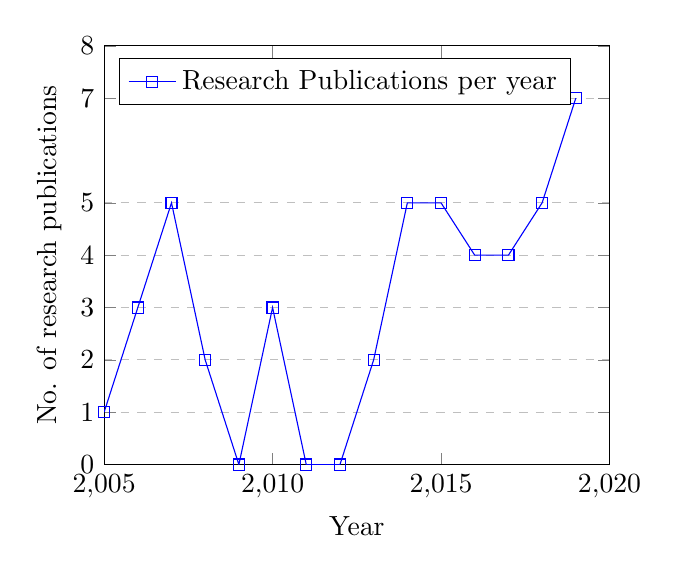
\begin{tikzpicture}
    \begin{axis}[
   %% title={Research on System and Network Fingerprinting},
    xlabel={Year},
    ylabel={No. of research publications},
    xmin=2005, xmax=2020,
    ymin=0, ymax=8,
    xtick={2005,2010,2015,2020},
    ytick={0,1,2,3,4,5,7,8},
    legend pos=north west,
    ymajorgrids=true,
    grid style=dashed,
    ]

    \addplot[
    color=blue,
    mark=square,
    ]
    coordinates {
    (2005,1)(2006,3)(2007,5)(2008,2)(2009,0)(2010,3)(2011,0)(2012,0)(2013,2)(2014,5)(2015,5)(2016,4)(2017,4)(2018,5)(2019,7)
    };
    \legend{Research Publications per year}
    
    \end{axis}
    \end{tikzpicture}
    \end{center}
    \label{graph:reseatch_per_year},
    \caption{Research on System and Network Fingerprinting}
   \end{figure} 
    

Identifying deviations in the behavior of a system and inferring fingerprints has been an active research topic. Early works by Brumley et al. \cite{Brumley} involved theoretical approach based on binary analysis. All attacks towards honeypots are recorded or logged for further analysis. This process is an expensive operation considering the writes and file operations thereby creating delay in the response times of the honeypot. Further, honeypots utilize the virtual environments to save resources in their environment. Based on these ideas, Holz et al \cite{Holz} proposed that honeypots could be detected due to increase in execution time of the commands from the attackers because of logging and sandboxing.Fu et al. \cite{Fu} also, suggested that the delay in execution and the response due to the virtualized network layer leveraged by honeypots could be a factor to infer the presence of the honeypot. At the Black Hat conference 2015, Cymmetria research \cite{BLACKHAT} proposed various factors by which honeypots could be fingerprinted and recommended new design strategies and development practices to overcome the detection. Alexander et al. \cite{Vetterl2018} provide a systematic fingerprinting approach for low-interaction honeypots. They leverage the faults of poorly maintained libraries referenced in the emulation of protocols in popular honeypots. The libraries used in the development of protocols in honeypots were not intended to reproduce the actual behavior of the protocol itself but used for the ease of development. The authors present a fingerprinting approach by development of probes that trigger the response at the transport layer and were successful in identifying up to 7605 honeypots online. Their research is limited to SSH, Telnet and HTTP honeypots. Internet scanning tools like Shodan have also released Honeypot identification methods called Honeyscore \cite{SHODAN}.The tool accepts an IP address or a URL as an input and provides result if the end system is a honeypot. The tool is stated to be still in development but is capable of recognizing popular honeypots on the internet. Feng et al. \cite{Feng2016} propose a machine learning model to collect and classify the response data received from Industrial Control Systems open on the internet. The approach relies on the flawed implementation of industrial control protocols and the deployment configurations of the honeypots. Figure \ref{graph:reseatch_per_year} shows the increasing research in the area of system fingerprinting over the years. Over the last five years, there is consistent increase for fingerprinting research techniques. 



\begin{table*}[ht!]
\caption{\label{tab:Table1}Protocols and Honeypots}
\centering
 \begin{tabular}{||c c c c c c c||} 
 \hline
 SSH & Telnet & HTTP & SMB & Database & ICS & IoT\\ [0.5ex] 
 \hline
 Kippo & Telnet-IOT-Honeypot & Dionaea & HoneySMB & mysql-honeypotd & Conpot & HoneyThing\\ 
 
 HosTaGe &  HosTaGe &  HosTaGe &  HosTaGe &  HosTaGe &  HosTaGe &  HosTaGe  \\
 
 Cowrie & Cowrie & Glastopf &  & pghoney & GasPot & Kako\\

 Blacknet & TPwd & Conpot &  & MongoDB-HoneyProxy & GridPot & IotPot\\
 
 Kojoney2 & MTPot & Nodepot & & & & \\
 
 MockSSH & Hontel &  &  & & & \\ [1ex] 
 \hline
\end{tabular}

\end{table*}


\section{Honeypot Fingerprinting Techniques}

Based on previous work, we now present various fingerprinting techniques for honeypots. The techniques are inferred from related work in the area of fingerprinting and contributions from researchers. Based on their type, we list four methods of fingerprinting of honeypots. 
The fingerprinting methods are explained in detail in further sub-sections. 

\subsection{Meta-Data based fingerprinting}
Meta data based fingerprinting leverages the basic known information about the honeypot. This method does not necessarily need any interaction with the honeypot to determine any information. The technique utilizes basic information like the IP address or the domain name to infer the probability of honeypot existence. With IP address information, it is possible to determine other meta data about the system like the geo-location, internet service provider, autonomous system , hosting or cloud provider. This meta data can be further analysed to determine the probabilities of a honeypot. For example, if the target system has the TCP port 500 open and is geo-located to be in an University, it can be possible that the target system is an honeypot. Another example would be if the same system is found to be hosted by a cloud provider like AWS, it is very likely that the system is a honeypot because Industrial Control Systems are physical devices that cannot be hosted or deployed on a cloud network.
Internet wide scanning tools like Shodan provide honeypot detection services. The service HoneyScore, accepts either an IP address or a URL to check in its database. Shodan describes that the service works by using the characteristics of known honeypots and assigning a score from 0.0 to 1.0 based on a match of the characteristics. The scores are stored in a native database. The service is still under development, but is capable of detecting popular honeypots listed in Table \ref{tab:Table1}. Shodan also provides an API that can be used to integrate in scanning or fingerprinting scripts. Other meta data based fingerprinting methods include using search engines to collect information about the target system. Popular search engines crawl through the internet on a daily basis to improve search results.With the search information, it is possible to identify and group relevant information to determine additional facts for the fingerprinting approach. Meta-data based fingerprinting is a passive fingerprinting approach.


Based on the information received from meta-data methods, it is possible to infer the existence of a honeypot with minimal interaction. We formulate the process of fingerprinting with the meta data approach based on the data received through the process. Figure 1 shows the formal approach to fingerprint honeypots with the meta data based method. The parameters like geolocation provide information about the location of the honeypot. This information can be used to find relevance to the services rendered by the honeypot. For example if the location is identified as an educational institution, it is very likely that the system is a honeypot deployed for experimental purposes. Similar inferences can be made with the data received from other parameters like ISP and hosting information. In the following subsections we provide further information about the information that can be derived using meta data. 
\newline
\subsubsection{Geo Location}
The location of a system determines what sector it is being used. It is possible to accurately determine the location of any system bearing a public IP address. This information is particularly useful when the system is suspected to be in a location which is not relevant for the services it is offering. This information can be used to derive that the target is either a training system or a honeypot. 
\newline
\subsubsection{Internet Service Provider}
With the IP address information, it is possible to find the Internet Service Provider that the address pool belongs. This is specially useful in deriving information about the service providers to industries and corporate environments. Normally, enterprises have dedicated lease lines or fiber lines from well known service providers. Also, it is quite possible that service providers deploy many honeypots in their management networks as a proactive defense strategy. For example, Deutsche Telekom has deployed TPot \cite{TPot}, a collection of known honeypots in its networks. TPot has also been a widely deployed honeypot for SSH ,Telnet and HTTP protocols. 
\newline
\subsubsection{Hosting Provider}
The hosting of the target system is a good evidence of implication of a honeypot. If the target is found to be hosted with a cloud provider, with pointless services, it is very conclusive that the target is a honeypot. Also, if the system is hosted with an unrelated domain pool which differs from the content of the honeypot, it can further lead to the inference of being a honeypot. It is very important for honeypot developers to create content and responses that relate to the hosting domain.  
\newline
\subsubsection{Search Engines}
Social Engineering is a leading Offensive Security strategy. Most of the findings from other attackers are documented or reported on fingerprinting databases. Searching the meta data with sensible parameters on an advanced internet search engine can provide interesting information about the target system. This information may include the past activity with the system, exploits, findings which can be used to infer that the target is an honeypot. The source of the information can be used in a scan script as a search database for fingerprinting. 
\newline
\subsubsection{Shodan Search}
Shodan is a database of vulnerable systems on the internet. It provides search as a service by accepting IP address, hostname or service names as search parameters. The output contains information about the target system and its open services. Shodan also provides a Honeypot Detection service called HoneyScore \cite{SHODAN} in addition to the database of vulnerable systems. Shodan performs daily scans of the internet with probe based fingerprinting methods to identify vulnerable systems on the internet. It has also a major source for attackers to get fast access to vulnerable systems. 
\newline
\subsection{Probe based fingerprinting}
Probe based fingerprinting involves creation of crafted queries to target devices to derive fingerprinting information. The probe based methods engage with  the target system unlike the meta data methods. These methods focus on leveraging the responses from communication protocols and classifying the target machine based on specific values from the responses. Constructing probes is an advanced method that requires proficient knowledge of systems and protocols. Therefore extensive knowledge about systems and protocols is necessary for probe based methods. The queries are constructed to trigger specific information from the target machine. The information may include system specific unique values for parameters like initial congestion window (ICW) or re-transmission timeouts (RTO). 
Shu et al.\cite{shu2006network} proposed fingerprinting of network protocols with a formal approach. The approach proposes a parameterized extended finite state machine (PEFSM) to formally model protocol specification and candidate conforming implementations. Several fingerprinting tools like NMap, Metasploit and Hydra make use probe based  methods to determine the operating systems and the protocol versions of the target systems. These tools rely on TCP packet information to determine the operating system. The specific values unique to each operating system are logged in  the tools database. This helps in comparison of the value of parameters obtained by probing and determine the operating system by matching the closed parameter value from the database. We discuss different probe based techniques in further subsections. 
\newline
\subsubsection{Port Scanning}
Port scanning is the most employed technique by attackers. It forms the first step before attacking a target system. Port scanning involves scanning and listing open ports on the target system. Ports which are open signify that they are open for communication and the active services on the system. Many administrators leave the services running on default ports and configuration. For example, port 22 is used for SSH and port 80 for HTTP web service. Port scanning provides information about the transport layer protocol used, the port number and the status of the port. Popular port scanning tools like NMap\cite{NMap} provide more information about the open ports like the active service, version and the vulnerabilities associated with the version. Nmap also provides fast scans and detailed scans. It recognises six port states and classifies them into open, closed, filtered, unfiltered, open-filtered and closed-filtered and has a database of fingerprinting information for 2000 services. 
Tools like NMap and ZMap \cite{zmap} provide parametrized scripts to run port scanning on target machines. Further, custom scripts are developed with NMap that can identify honeypots like Kippo and Dionaea.  
\newline
\subsubsection{Banner Grabbing}
Banner grabbing is one of the techniques used in reconnaissance process following a port scan. After learning about the open ports, a connection is established with the remote system to get information about the service and the version number. Some implementations of protocols like FTP and HTTP expose critical system information like service name, software, version and the operating system. Banner grabbing based probes targeted on a protocol can reveal vulnerabilities associated with any critical information obtained. The CVE database \cite{CVE} provides a list of vulnerabilities associated with respect to protocols, software and operating systems. Popular tools for Banner Grabbing are Wget, cURL, NMap, Netcat, and Dmitry. Banner grabbing is an integrated feature with port scanning on most of the port scanning tools.  
\newline
\subsubsection{Handshake Proposals}
TLS handshake is a process that establishes the parameters for secure communication between systems. The handshake process involves exchange of messages to acknowledge each other, TLS version,  negotiate the cipher suites, authentication with the public key and session keys generation. In addition there are parameters like message size and timestamp. TLS negotiations are transmitted in clear text. With the information available through this negotiation, it is possible to fingerprint the client and server applications.  The handshakes also determine the cipher suites proposed by the target system. This information can be leveraged to find vulnerabilities and to characterize the systems based on limited choice of ciphers. JA3 and JA3s\cite{JA3} are techniques developed that can actively fingerprint the TLS client and servers based on their hello messages.
\newline
\subsubsection{Deep Packet Inspection}
Deep packet inspection(DPI) is a method for analysing and monitoring network traffic. Using DPI, network packets can be filtered based on the protocol type and the data in packet components. Conventional packet inspection methods examine only the header information for filtering the traffic. DPI is performed at enterprises using layer 6 devices like firewalls or intrusion detection systems. DPI can help to identify redundant responses received from a machine for fingerprinting purposes. DPI relies on a repository of existing protocol fingerprints for classification. It is an effective technique used by intrusion detection systems to filter malicious packets from the production networks. On the contrary, DPI can be an effective technique to fingerprint end systems or protocols based on the header and the payload information. Sang et al.\cite{Sang} proposed a fingerprinting technique based on byte embedding for classification of network protocols. The approach learns the application fingerprints from traffic traces by characterizing the packet payloads with byte embedding based payload alignment algorithm. However, with open-source libraries and tools like nDPI\cite{nDPI} it is possible to fingerprint and inspect various protocols. DPI requires good knowledge of packet level communication and networking. It is an advanced probe based method which requires advanced knowledge for creation of probes to retrieve specific information from the target system. 
\newline

\subsubsection{Default Configuration Check}
Applications are setup with setup scripts or by using install media. Often, these media do not prompt the user to change the default settings or configuration prior to final installation. This leaves the system running with a default configuration. For example, we have Apache Tomcat Manager instance running on a default installation of Apache Tomcat. The manager provides an interface to manage the web service and the deployments. It is important to configure the tomcat manager or disable if not used. Similarly, there are devices and applications running with default configurations on the internet. With these default configurations, it is easily possible to  fingerprint the target system. Honeypots like Kippo, Cowrie, Glastopf and Conpot are usually deployed with default configurations. Morishita et al. \cite{morishita} provide an approach to self revealing honeypots on the internet by detection through default configurations.  This leads to easy discovery of honeypots by constructing a probe to check the default configuration. If the response matches the defaults, the end systems is likely a honeypot. 
\newline

\subsubsection{System information}


\newline

\subsubsection{Sniffing}

\newline
\subsubsection{Multi-stage attacks}

\newline
However, there are risks involved in probe based fingerprinting methods. As these methods involve direct interaction with the target system, eventually the probe system is blacklisted. We must remember that there is no real reason for establishing a connection with a honeypot. Any connections observed with a honeypot is considered potentially an attack. Probing systems may get blocked by this approach. This limits in further exploitation or identification of the attacker or the honeypot. It is important to keep the attacker engaged with the honeypot to collect as much possible to identify the attacker. 


\subsection{Dependency based fingerprinting}


\subsection{Machine Learning based fingerprinting}









 \section{Classifying Honeypot Fingerprinting Methods}
   
   Fingerprinting methods are basically classified into active and passive based on interaction with the target system. Active fingerprinting involves creation of specific probes and using them to query the the target system to collect as much data possible. On the contrary, passive fingerprinting  make use of sniffing traffic or basic packet inspection to determine information about the target. Passive fingerprinting limit communication with the target system as much possible. Remote attackers tend to use active fingerprinting methods as passive fingerprinting requires the use of a sniffing tool deployed on the network of the target system. Passive fingerprinting techniques depend on fingerprint databases to infer their findings. Fingerprint databases contain information about distinct responses by systems on interaction. These responses may involve TTL (Time to Live) for specific flags in an ICMP response. Such methods are used to determine the operating system or the versions of the network protocols on the target system.
   
   Concentrating fingerprinting methods on honeypots, we propose an approach based on interaction methods. This is important as the many honeypot networks block communication with the attackers after a connection attempt. This limits the detection and further exploitation of the honeypot and the system. Also, we believe to use minimum interaction with the honeypots for fingerprinting, to limit logging information about the attacker. 


 \section{Evaluation of Honeypots based on Classification}
 
 
 
 \section {Countermeasures}
 
 
 
 \section {Related Work}
 
 
 
\section{CONCLUSIONS}


\addtolength{\textheight}{-12cm}   % This command serves to balance the column lengths
                                  % on the last page of the document manually. It shortens
                                  % the textheight of the last page by a suitable amount.
                                  % This command does not take effect until the next page
                                  % so it should come on the page before the last. Make
                                  % sure that you do not shorten the textheight too much.

%%%%%%%%%%%%%%%%%%%%%%%%%%%%%%%%%%%%%%%%%%%%%%%%%%%%%%%%%%%%%%%%%%%%%%%%%%%%%%%%



%%%%%%%%%%%%%%%%%%%%%%%%%%%%%%%%%%%%%%%%%%%%%%%%%%%%%%%%%%%%%%%%%%%%%%%%%%%%%%%%



%%%%%%%%%%%%%%%%%%%%%%%%%%%%%%%%%%%%%%%%%%%%%%%%%%%%%%%%%%%%%%%%%%%%%%%%%%%%%%%%

\section*{ACKNOWLEDGMENT}




%%%%%%%%%%%%%%%%%%%%%%%%%%%%%%%%%%%%%%%%%%%%%%%%%%%%%%%%%%%%%%%%%%%%%%%%%%%%%%%%



\bibliographystyle{plain}

\bibliography{references}



\end{document}
